\clearpage
\section{Instrukcja użytykownika}
\label{sec:manual}

\quad Jak zostało wcześniej wspomniane, możliwość interakcji z systemem silników została przewidziana w formie dwóch aplikacji. Niniejszy rozdział został poświęcony opisowi możliwych schematów wykorzystania przygotowanego oprogramowania. Podstawą obu jest opisywana w rozdziale \ref{sec:spec_prog} biblioteka Taurus, a konkretniej jej część (o nazwie ,,TaurusGUI'') umożliwiająca programowanie bądź konfigurację głównych okien interfejsów użytkownika.

\subsection{Aplikacja ekspercka}
\label{sub:expertgui}

\quad Pierwsza z utworzonych aplikacji to interfejs ekspercki - został on przedstawiony na rysunku \ref{fig:ExpertGUI}. Umożliwia on sprawowanie pełnej kontroli nad procesem sterowania silnikami, a więc również nad przeprowadzaniem eksperymentów na linii badawczej. Została ona podzielona na 4 części oraz dwa menu:

\begin{enumerate}
	\item Część w lewym górnym rogu zawiera dwa panele. Pierwszy o nazwie ,,Macros'', widoczny na rysunku przedstawiającym aplikację ekspercką, to panel umożliwiający użytkownikowi wybór odpowiedniej, pojedynczej komendy spośród obfitego zestawu dostępnych, ustawienie jej parametrów i uruchomienie. Wybór odbywa się poprzez kliknięcie odpowiedniej pozycji na rozwijanej liście. Uruchomić makro można przyciskiem ,,Play'' - obok niego znajdują się również przyciski do wstrzymywania i przerywania działania komendy. Dioda w ostatnim wierszu pokazuje stan urządzenia, które zajmuje się wykonywaniem makr - kolory odpowiadają standardom Tango, opisanym w rozdziale \ref{sec:spec_prog}.
	
	Drugi panel - ,,Macro Description'' - zawiera opis wybranego makra. Przedstawia on skrótowy opis działania komendy oraz znaczenie i zakres wszystkich jej parametrów - zarówno wejściowych, jak i wyjściowych (jeśli dane makro cokolwiek zwraca). Znajdują się tam również czasem dodatkowe informacje lub fakty, na które warto zwrócić uwagę. Wyboru można dokonywać zarówno na poprzednim panelu w tej części aplikacji, jak i na panelu ,,Sequence'', opisanym niżej.
	
	\item Część w prawym górnym rogu zawiera aż 4 panele. Pierwszy z nich, widoczny na rysunku, to panel ,,Sequence''. Zawiera on opcje pozwalające na wykonywanie, zapisywanie i wczytywanie sekwencji makr. Pierwsza z tych operacji jest aktywowana przyciskiem ,,Play'', podobnie, jak na panelu ,,Macros'' (jak również przyciski umożliwiające wstrzymanie i przerwanie działania makra). Możliwość tworzenia nowej sekwencji, otwierania istniejącej i zapisywania bieżącej dają (w takiej właśnie kolejności) przyciski, które znajdują się w górnym lewym rogu panelu.
	
	Po wybraniu makra z rozwijanej listy można je dodać do edytowanej sekwencji przyciskiem ,,+'' znajdującym się w prawym górnym rogu panelu. Przyciski poniżej ,,+'' umożliwiają odpowiednio usunięcie makra z sekwencji, przesunięcie go w górę lub w dół na liście obrazującej kolejność wykonywania oraz zmianę poziomu wykonywania makra (dotyczy tylko niektórych, powiązanych komend). Po wybraniu makra na liście sekwencji uaktywnia się dolna lista na panelu, która zawiera konfigurację wszystkich argumentów wejściowych makra.
	
	Pozostałe panele w tej części aplikacji eksperckiej - ,,DoorOutput'', ,,DoorDebug'' oraz ,,DoorResult'' - zawierają informacje zwrotne uzyskiwane po uruchomieniu makra (bądź ich sekwencji). Znajdują się tam odpowiednio komunikaty, wiadomości dotyczące odpluskwiania makra (jeśli uruchomione jest ono w takim trybie) oraz wyniki ewentualnych obliczeń. W przygotowanej na potrzeby sekwencji makr te panele nie są wykorzystywane.
	
	\item Część znajdująca się w lewym dolnym rogu zawiera tylko jeden panel - ,,Positions''. Jest on interaktywnym wykresem, aktualizowanym na bieżąco w czasie rzeczywistym (okres oczekiwania na odświeżenie wynosi 1 do 3 sekund). Zmiennymi, których wartości przedstawia są położenia wszystkich czterech silników, stanowiących podstawę niniejszego projektu. Ten panel daje użytkownikowi bardzo dużo możliwości - większość z nich jest dostępna poprzez kliknięcie prawym przyciskiem myszy na wykres. Pokazuje się wtedy menu kontekstowe, które zawiera takie opcje, jak:
	\begin{itemize}
		\item dostosowywanie ustawień osi (wybór zakresów, zmiana trybu z liniowego na logarytmiczny, określenie kolorów odpowiadających poszczególnym sygnałom, itp.),
		\item ustawienie zmiennych prezentowanych na wykresie,
		\item zapisanie i wczytanie aktualnych ustawień wykresu,
		\item zmianę tytułu,
		\item dostosowanie skal osi (oraz opcję autoskalowania),
		\item włączanie/wyłączanie pokazywania wartości minimalnej/maksymalnej oraz legendy,
		\item obliczanie większej ilości parametrów statystycznych.
	\end{itemize}
	Dodatkowo, klikanie na nazwy atrybutów w legendzie pozwala wyłączać pokazywanie odpowiadającej im krzywej na wykresie lub przełączanie się między prawą i lewą osią Y.
	
	\item W prawym dolnym rogu aplikacji eksperckiej znajdują się dwa panele - ,,/slit'' oraz ,,/mirror''. Oba umożliwiają bezpośrednie poruszanie silnikami bądź grupami silników. Każdy z nich zawiera pola do wpisywania wartości zadanych oraz monitorowania aktualnego położenia silników. Przycisk ,,Stop'', znajdujący się między polami każdego silnika pozwala zatrzymać ruch. Po lewej stronie, zaraz za nazwą silnika, znajdują się przyciski ,,-'' oraz ,,+''. Pozwalają one na wykonanie pojedynczego kroku odpowiednim silnikiem.
	
	Kluczową sprawą dla użytkowania aplikacji jest zwracanie uwagi na format wpisywanych w polach edycyjnych danych. Normalna czcionka oznacza brak różnic między wartością zadaną a aktualnym położeniem. W takim stylu są też wyświetlane wartości po uruchomieniu aplikacji. Kolor niebieski i pogrubienie czcionki znamionują obecność takich zmian - można je zatwierdzić, używając klawisza Enter. Użytkownik może również chcieć zaaplikować wartość wyświetlaną w normalnym stylu (na czarno) - w tym celu przewidziano kombinację klawiszy Ctrl + Enter. Żółty kolor czcionki oznacza wartość, która przekroczyła poziom ostrzeżenia. Kolor żółty oraz czerwona ramka naokoło pola edytowalnego - wartość przekraczającą poziom alarmowy.
	
	\item Dodatkowymi elementami aplikacji są 2 menu oraz dioda znajdująca się w prawym dolnym rogu. Jej ciągłe miganie to efekt ,,bicia serca'' (ang. hearbeat), czyli proste sprawdzenie, czy aplikacja działa, czy się zacięła.
	
	Pierwsze menu znajduje się na samej górze aplikacji. Składa się z dwóch części - jedna to standardowe menu aplikacji, w którym znajdziemy takie opcje jak zapisanie perspektywy, zmianę widoku, opcje wyświetlania i ukrywania paneli, itp. Poniżej znajdują się przyciski menu narzędziowego - umożliwiają one szybki dostęp do maksymalizacji okna, wczytania perspektywy (czyli aktualnie wyświetlanej konfiguracji paneli) oraz dodanie nowego panelu.
	
	Drugie menu znajduje się w pasku po prawej stronie aplikacji. Obecne tam 4 ikony to odpowiednio - logo organizacji, logo aplikacji, przycisk paniki (zatrzymuje wszystkie aktualnie wykonywane operacje) oraz tryb inspekcji.
\end{enumerate}


\begin{figure}[ht]
	\begin{adjustbox}{addcode={
				\begin{minipage}{\width}}
					{\caption{Zrzut ekranu pokazujący aplikację ekspercką.}\label{fig:ExpertGUI}
				\end{minipage}},rotate=90,center}
		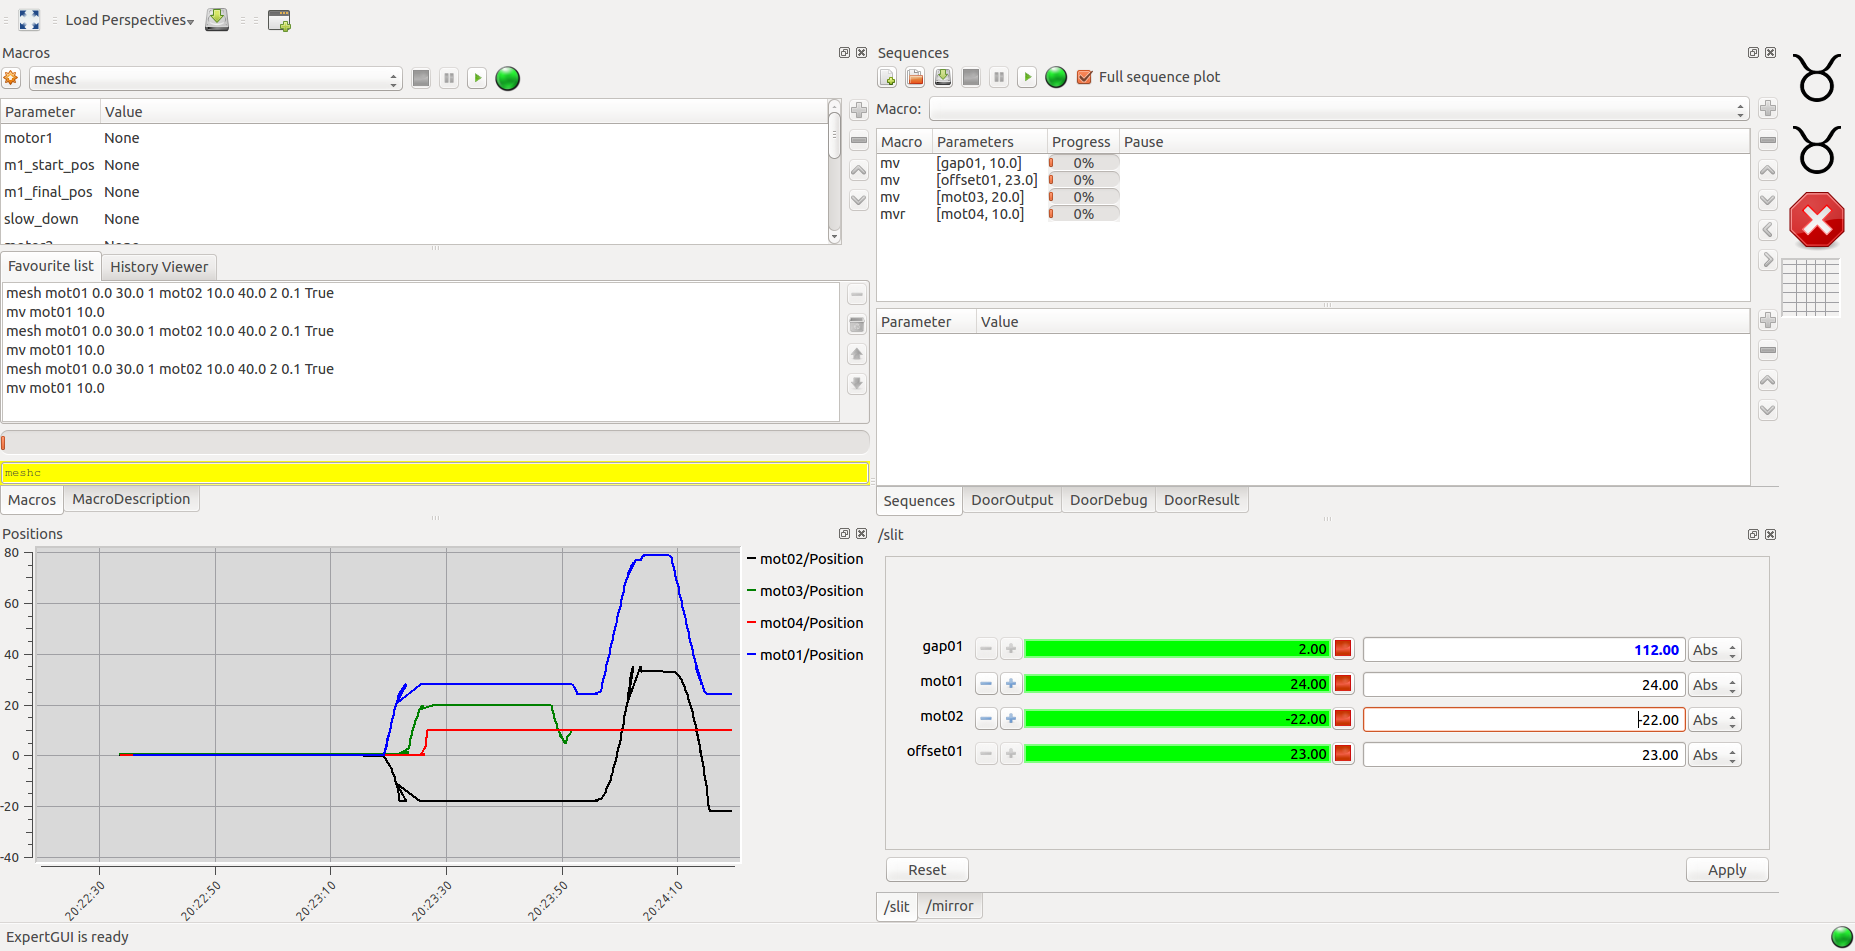
\includegraphics[scale=.32]{Grafika/ExpertGUI}
	\end{adjustbox}
\end{figure}

Przykładowe użycie aplikacji mogłoby obejmować następujące kroki:
\begin{enumerate}
	\item Uruchom aplikację poprzez wywołanie skryptu: \texttt{./ExpertGUI}.
	\item Wczytaj zapisaną perspektywę, sekwencję makr i ustawienia wykresów.
	\item Sprawdź, czy wszystko jest gotowe do przeprowadzenia eksperymentu (w szczególności należy zadbać o właściwą kolejność makr i odpowiednie dla nich argumenty).
	\item Włącz sekwencję makr.
	\item Monitoruj położenie silników na wykresie.
	\item W razie potrzeby, dopasuj ręcznie pozycję (lub zostaw to operatorowi).
\end{enumerate}


%---------------------------------------------------------------------------------------------------
\subsection{Aplikacja kliencka}
\label{sub:operatorgui}

\quad Druga z utworzonych aplikacji to interfejs klienta lub operatora - jest on przedstawiony na rysunku \ref{fig:OperatorGUI}. Pozwala on tylko na poruszanie konkretnymi silnikami w - operator może skorygować w niewielkim zakresie wartość położenia każdego elementu ruchomego i zobaczyć aktualny stan poszczególnych silników.

Ta aplikacja zawiera tylko jeden typ panelu - taki sam dla wszystkich czterech silników, którymi operator może sterować. Każdy z tych paneli zawiera następujące elementy:
\begin{enumerate}
	\item Nazwę silnika (według konwencji Tango).
	\item Diodę określającą stan urządzenia (odpowiadającą standardowej kolorystyce wykorzystywanej w Tango). Na rysunku \ref{fig:OperatorGUI} są widoczne trzy możliwe stany urządzenia związanego z silnikiem.
	\item Duże, zielone pole statusu. Jego rozmiar jest warunkowany najdłuższym możliwym komunikatem, który jest w nim wyświetlany. Jak widać na rysunku \ref{fig:OperatorGUI}, może prezentować różne rodzaje informacji statusowej.
	\item Wykres kołowy aktualizowany na bieżąco, który pokazuje pozycję silnika.
	\item Pole edytowalne służące do wpisywania pożądanej wartości zadanej położenia silnika. Podlega dokładnie takim samym regułom, jak to w aplikacji eksperckiej, opisane w podrozdziale \ref{sub:expertgui}.
\end{enumerate}

Najechanie kursorem na dowolny element powyższej listy (oprócz nazwy silnika) powoduje pokazanie się widocznej na rysunku \ref{fig:OperatorGUI} podpowiedzi dotyczącej atrybutu dołączonego do danego elementu aplikacji. W przypadku pozycji pokazują się tam takie informacje, jak zakres, poziomy ostrzeżenia i alarmu.

Aplikacja operatora, tak jak opisywane wcześniej oprogramowanie eksperta, posiada menu bazowe aplikacji opartej o TaurusGUI, a więc umożliwiające m.in. konfigurację widoku oraz tworzenie perspektyw.

Przykładowy proces korzystania z aplikacji może być przedstawiony w następujących krokach:
\begin{enumerate}
	\item Uruchom aplikację poleceniem: \texttt{python OperatoGUI/operator\_gui.py}
	\item Sprawdź, czy stany wszystkich silników umożliwiają poruszenie nimi.
	\item Dokonaj odpowiednich korekt w położeniu.
\end{enumerate}


\begin{figure}[ht]
	\begin{adjustbox}{addcode={
				\begin{minipage}{\width}}
					{\caption{Zrzut ekranu pokazujący aplikację operatora.}\label{fig:OperatorGUI}
				\end{minipage}},rotate=90,center}
				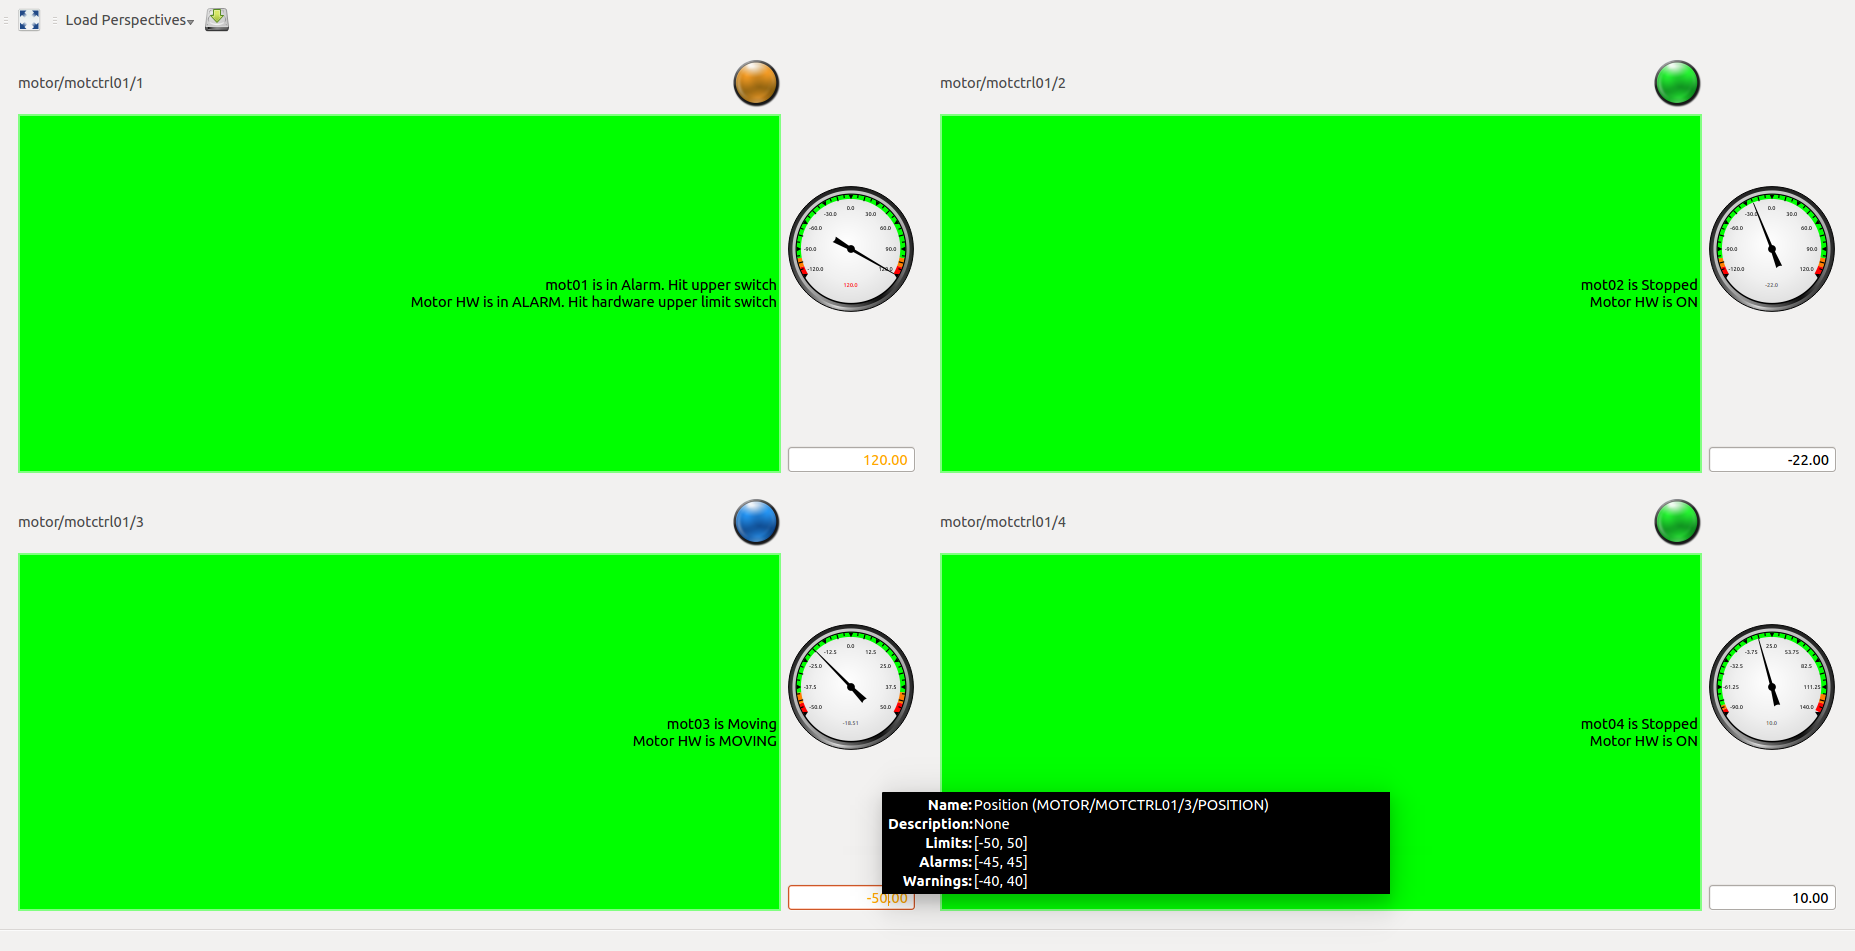
\includegraphics[scale=.32]{Grafika/OperatorGUI}
	\end{adjustbox}
\end{figure}